%%%%%%%%%%%%%%%%%%%%%%%%%%%%%%%%%%%%%
% This file is the "main" or root file for the book. It describes what packages
% and content should be included in what order.

\documentclass[pagesize=auto,bibliography=totocnumbered]{scrbook}

\usepackage{comment}
\usepackage{etoolbox}
\usepackage{fancyvrb}
\usepackage{graphicx}
\usepackage{hyperref}
\usepackage[round]{natbib}
\usepackage{xspace}
\usepackage{xcolor}

% This is for multilingual work. Would be nice to support Chinese and Thai.
\usepackage[T2A]{fontenc}
\usepackage[utf8]{inputenc}
\usepackage[greek,russian,english]{babel}
\usepackage{amsthm}
\usepackage{amsmath}
\usepackage{amssymb}
\usepackage[linesnumbered,algoruled,boxed,lined]{algorithm2e}
\usepackage{hyperref} % This package is needed for \texorpdfstring

% This file is for commands / macros / functions.

% That at least was the original intention. As you can see from the comments, some of the commands
% that work for TeX and pdf output are innefective when applied to HTML and eBooks!

% These are useful because HTML output corrupts the result of the \latex command.
\newcommand{\latex}{LaTeX\xspace}
\newcommand{\tex}{TeX\xspace}

% Makes extra space in HTML but not in PDF output.
\def\htbr{\ifdefined\HCode{\HCode{<br/><br/>}}\fi}

\newcommand\nextpage[1][]{
\ifdefined\HCode {
  \HCode{<mbp:pagebreak />}}
\else
  \newpage
\fi
}

% Makes small typewriter text, comparable to other font sizes.
\def\smalltt#1{\texttt{\small #1}}

% Makes small verbatim inline typewriter text, comparable to other font sizes.
% Use as \sverb|My verbatim text|
\def\sverb{\Verb[fontsize=\small]}

% Makes small URL text, comparable to other font sizes.
\def\surl#1{{\small{\url{#1}}}}
\newtheorem{theorem}{Theorem}
\newtheorem{definition}{Definition}
\newtheorem{lemma}{Lemma}
\newtheorem{proposition}{Proposition} 
\newtheorem{corollary}{Corollary} 
\newtheorem{remark}{Remark}


% This line stops the insertion of extra blank pages between chapters.
\ifdefined\HCode{\KOMAoptions{twoside=false}} \fi

\begin{document}

% Title and author are written down in the cover_page.tex file, and author
% appears also as an argument to the ebook-convert command in the build.sh file.
%% This is a cover page.

\thispagestyle{empty}

\vspace{3cm}
  \begin{center}
	\bfseries \Huge Theorem-You-Must-Know \par   % Your own title would go here.
        ~\\
	\bfseries \LARGE Some theorem proofs related to Cryptography or computational number theory. \\   % Include a subtitle or just delete.
        ~\\
        \bfseries \Large @fffmath \par   % The author's name goes here.

        \vspace{3cm}
    
      	{\centering 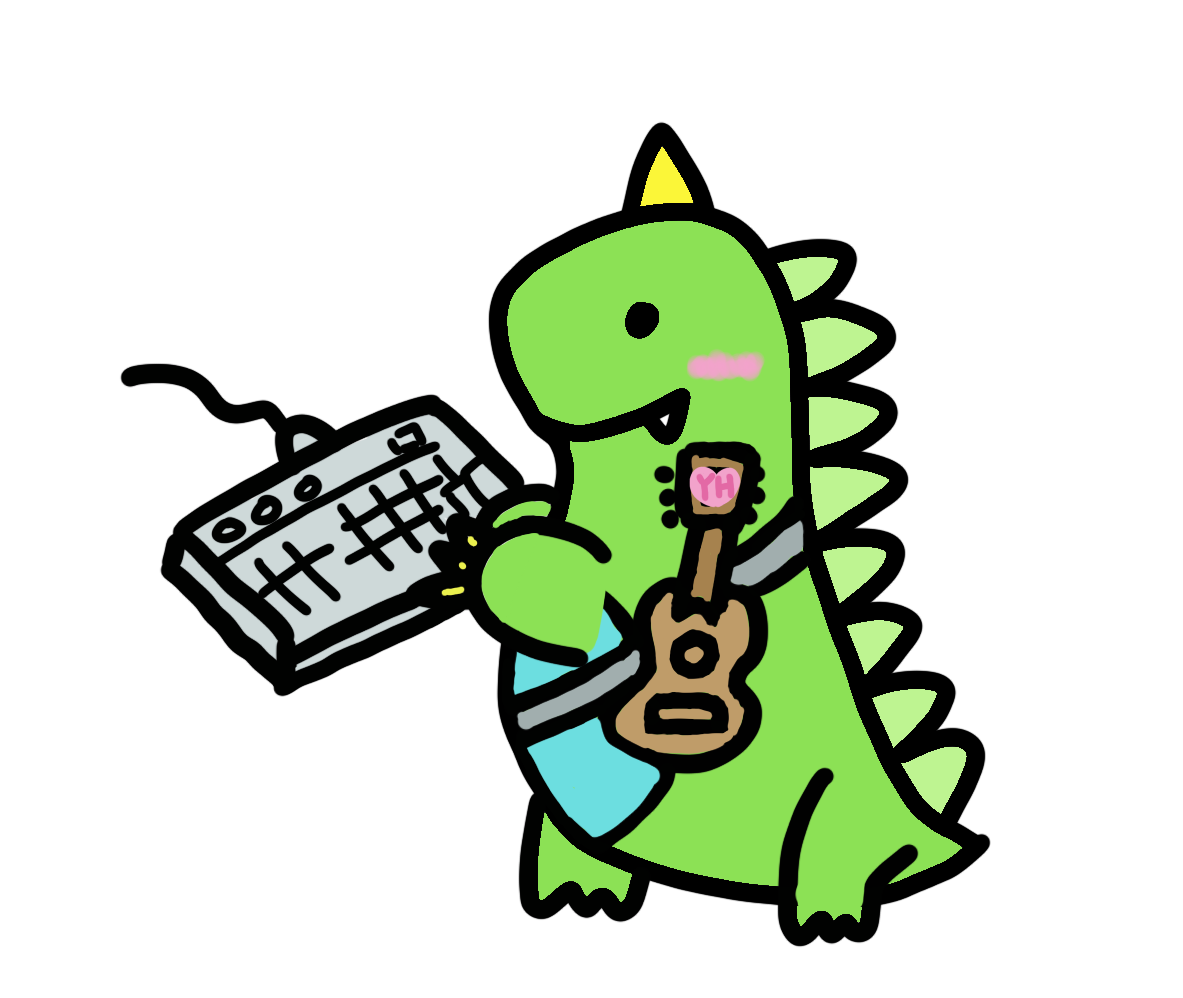
\includegraphics[width=0.8\linewidth]{images/myavatar.png}}
    \end{center}
    
\par

\newpage


\tableofcontents

\nextpage
%% Introduction / first chapter.

\chapter{Introduction}

The original \tex was created by the famous computer scientist Donald Knuth \citep{knuth1984texbook},
and added to by Leslie Lamport to make \latex \citep{lamport1985latex}.

%%%
\section{How to Use this Book}
These are the main ways you can use this material:

\begin{itemize}
    \item Lattice
    \item Zero-Knowledge Proof
    \item You can use it as a template. All of the source files used to make this book
    are freely available in GitHub at {\small \url{https://github.com/dwiddows/ebookbook}} and Overleaf.
    The source files are laid out in a way that should make it easy to clone the project and adapt it for your own book.
\end{itemize}

%% Lattice 

\chapter{Lattice Based Cryptography}
\section{Basic of lattice}
\subsection{The two definitions of lattice are equivalent}
\begin{definition}[Lattice]~\label{lattice1}
Given $n$ linearly independent vectors $\mathbf{b}_1, \ldots, \mathbf{b}_n \in \mathbb{R}^m$, the lattice generated by them is defined as
$$
\mathbb{L}(\mathbf{b}_1, \ldots, \mathbf{b}_n) = \left\{ \sum_{i=1}^{n} x_i \mathbf{b}_i \ \bigg| \ x_i \in \mathbb{Z} \right\}
$$
\end{definition}
\begin{definition}~\label{lattice2}
    A lattice $\mathbb{L}$ is a discrete additive subgroup of $\mathbb{R}^n$.
\end{definition}
\begin{theorem}
        The two definitions of lattice are equivalent.
\end{theorem}
\begin{proof}
    We will first show that Definition \ref*{lattice1} $\Rightarrow$ Definition \ref*{lattice2}.

    Assume $\mathbb{L}$ is a lattice defined as the set of all integer combinations of vectors $\mathbf{b}_1, \ldots, \mathbf{b}_n \in \mathbb{R}^m$ which are linearly independent (Definition 1). Then, clearly $L$ is an additive subgroup of $\mathbb{R}^n$. In addition, $\forall \mathbf{x}, \mathbf{y} \in L$, $\mathbf{x} - \mathbf{y} \in L$. Therefore, from the lower bound on a shortest lattice vector, 
    $$\|\mathbf{x} - \mathbf{y}\| \geq \lambda_1(\mathbb{L}) \geq \min_{i=1,\ldots,n} \|\tilde{\mathbf{b}}_i\|.$$
    In other words, the length of any lattice vector must be greater than the length of a shortest lattice vector.
    Therefore, we can let $\varepsilon = \lambda_1$. So, both properties of Definition 2 are satisfied ($L$ is a discrete additive subgroup of $\mathbb{R}^n$).
    
    We show that Definition \ref*{lattice2} $\Rightarrow$ Definition \ref*{lattice1}. Given a discrete additive subgroup $L$ of $\mathbb{R}^n$, we construct a set of basis using the algorithm below.
    
    We will use the following definition of a closed parallelepiped:
    
    Given \(n\) linearly independent vectors \(\mathbf{b}_1, \ldots, \mathbf{b}_n \in \mathbb{R}^m\), their closed fundamental parallelepiped is defined as
\[
\overline{P}(\mathbf{b}_1, \ldots, \mathbf{b}_n) = \left\{ \sum_{i=1}^{n} x_i \mathbf{b}_i \ \bigg| \ x_i \in \mathbb{R}, 0 \leq x_i \leq 1 \right\}
\]

Pick \(\mathbf{y} \in \mathbb{L}\) such that there is no lattice vector between the zero vector and \(\mathbf{y}\). Let \(\mathbf{b}_1 = \mathbf{y}\).
Iterate for all \(i\), \(1 \leq i < n\): Assume we have already chosen \(\mathbf{b}_1, \ldots, \mathbf{b}_i\). Choose \(\mathbf{y}\) not in the span of \(\mathbf{b}_1, \ldots, \mathbf{b}_i\).
Consider a \(\overline{P}(\mathbf{b}_1, \ldots, \mathbf{b}_i, \mathbf{y})\) (See Figure-1 for an example).
Now, \(\overline{P}\) contains at least one lattice point (namely \(\mathbf{y}\)) and it contains finitely many lattice points. Now, choose a vector \(\mathbf{z} \in \overline{P}(\mathbf{b}_1, \ldots, \mathbf{b}_i, \mathbf{y}) \setminus \text{Span}(\mathbf{b}_1, \ldots, \mathbf{b}_i)\) such that \(\text{dist}(\mathbf{z}, \text{Span}(\mathbf{b}_1, \ldots, \mathbf{b}_i))\) is the smallest.

Note that we can do this since we have only finitely many points to choose from. Let \(\mathbf{b}_{i+1} = \mathbf{z}\).

We will now show that the above algorithm returns a basis \(\mathbf{b}_1, \ldots, \mathbf{b}_n \in \mathbb{R}^m\) for the lattice. Clearly, all \(\mathbf{b}_i\)s are in \(\mathbb{R}^m\) and they are linearly independent by the algorithm that we used. We are left to show that \(L \subseteq \left\{ \sum x_i \mathbf{b}_i : x_i \in \mathbb{Z} \right\}\).

Let \(\mathbf{z} = \sum z_i \mathbf{b}_i\) be an arbitrary lattice vector (where \(z_i \in \mathbb{R}\)). Let \(\mathbf{z}_0 = \sum b_z^i \mathbf{c}_i\) be an element of \(L\). Then, \(\mathbf{z} - \mathbf{z}_0 = \sum (z_i - b_z^i c_i) \mathbf{b}_i\) is in \(L\). We will show that all coefficients \(z_i\) must be integers. Express 
$$
\mathbf{z} - \mathbf{z}_0 = (z_n - \lfloor z_n \rfloor) \mathbf{b}_n + \text{Span}(\mathbf{b}_1, \ldots, \mathbf{b}_{n-1}) = (z_n - \lfloor z_n \rfloor) \mathbf{b}_n + \text{Span}(\mathbf{b}_1, \ldots, \mathbf{b}_{n-1}).
$$
In other words, vector \(\mathbf{z} - \mathbf{z}_0\) is in the span of \(\mathbf{b}_1, \ldots, \mathbf{b}_{n-1}\) plus a multiple of \(\tilde{\mathbf{b}}_n\) with coefficients \(0 \leq b_z^n c_n < 1\).

Now,
\[
\text{dist}(\mathbf{z} - \mathbf{z}_0, \text{Span}(\mathbf{b}_1, \ldots, \mathbf{b}_{n-1})) = (z_n - \lfloor b_n \rfloor) \|\tilde{\mathbf{b}}_n\|.
\]
This follows because the distance is defined as the orthogonal component of \(\mathbf{z} - \mathbf{z}_0\) to the span \(\text{Span}(\mathbf{b}_1, \ldots, \mathbf{b}_{n-1})\), which is precisely \((z_n - b_z^n c_n) \|\tilde{\mathbf{b}}_n\|\). Similarly,
\[
\text{dist}(\mathbf{b}_n, \text{Span}(\mathbf{b}_1, \ldots, \mathbf{b}_{n-1})) = \|\tilde{\mathbf{b}}_n\|.
\]
In addition, since \(0 \leq (z_n - b_z^n c_n) < 1\),
\[
\text{dist}(\mathbf{z} - \mathbf{z}_0, \text{Span}(\mathbf{b}_1, \ldots, \mathbf{b}_{n-1})) < \text{dist}(\mathbf{b}_n, \text{Span}(\mathbf{b}_1, \ldots, \mathbf{b}_{n-1})).
\]
But since \(\mathbf{b}_n\) was chosen as the closest vector to \(\text{Span}(\mathbf{b}_1, \ldots, \mathbf{b}_{n-1})\), \(\mathbf{z} - \mathbf{z}_0\) must be linearly dependent on \(\mathbf{b}_1, \ldots, \mathbf{b}_{n-1}\). Therefore, \(z_n - \lfloor b_n \rfloor= 0\) and so \(z_n \in \mathbb{Z}\).

By recursively repeating the above argument for \(\mathbf{z} = \mathbf{z} - \mathbf{z}_i \in \text{Span}(\mathbf{b}_1, \ldots, \mathbf{b}_{i-1})\) for all \(1 < i \leq n\), we obtain that all coefficients \(z_j\) for \(1 \leq j \leq n\) must be integers.

\end{proof}

\subsection{Complexity of LLL-algorithm}
\begin{theorem}
    Given an integer $n$-dimensional lattice basis with vectors of Euclidean norm less than $B$ in an $n$-dimensional space, the LLL algorithm outputs a reduced basis in $O(n^4 \log B \cdot M(n \log B))$ bit operations, where $M(k)$ denotes the time required to multiply $k$-bit integers.
\end{theorem}
\begin{proof}
    Our analysis consists of two steps. First, we bound the number of iterations. Second, we bound the running time of a single iteration.

We show that the overall running time of the algorithm is polynomial in the input size. A rough lower bound on the latter is given by $N := \max(n, \log(\max_i kb_i))$ (because each of the $n$ vectors requires at least one bit to represent, and a vector of norm $r$ requires at least $\log r$ bits to represent).

In the following, we show that the running time of the algorithm is polynomial in $M$. Moreover, the LLL algorithm outputs a reduced basis in $O(n^4 \log B \cdot M(n \log B))$ bit operations, where $M(k)$ denotes the time required to multiply $k$-bit integers.
\begin{algorithm}
    \caption{$\delta$-LLL Algorithm}
    \label{alg:delta-LLL}
    
    \KwData{Lattice basis $b_1, \ldots, b_n \in \mathbb{Z}^n$}
    \KwResult{$\delta$-LLL-reduced basis for $L(B)$}
    
    \BlankLine
    Compute $\tilde{b}_1, \ldots, \tilde{b}_n$\;
    
    \BlankLine
    \For{$i = 2$ to $n$}{
        \For{$j = i - 1$ to $1$}{
            $c_{i,j} \gets \frac{d \cdot \langle b_i, \tilde{b}_j \rangle}{\|\tilde{b}_j\|^2}$\;
            $b_i \gets b_i - c_{i,j} \cdot b_j$\;
        }
        Compute $\tilde{b}_i$\;
        
        \BlankLine
        \If{$\exists i$ s.t. $\delta k \tilde{b}_i^2 > k \mu_{i+1,i} \tilde{b}_i + \tilde{b}_{i+1}^2$}{
            Swap $b_i \leftrightarrow b_{i+1}$\;
            \textbf{goto Start}\;
        }
    }
    
    \BlankLine
    Output $b_1, \ldots, b_n$
    \end{algorithm}

    If the LLL algorithm terminates, it is clear that the output basis is LLL-reduced. What is less clear a priori is why this algorithm has a polynomial-time complexity. A standard argument shows that each swap decreases the quantity $\Delta = \prod_{i=1}^{n} \lVert b_i^* \rVert^2 (n - i + 1)$ by at least a factor $\delta < 1$. On the other hand, we have that $\Delta \geq 1$ because the $b_i$'s are integer vectors and $\Delta$ can be viewed as a product of squared volumes of lattices spanned by some subsets of the $b_i$'s. This proves that there can be no more than $O(n^2 \log B)$ swaps, and therefore loop iterations, where $B$ is an upper bound on the norms of the input basis vectors.

    It remains to estimate the cost of each loop iteration. This cost turns out to be dominated by $O(n^2)$ arithmetic operations on the basis matrix and GSO coefficients $\mu_{i,j}$ and $r_{i,i}$, which are rational numbers of bit-length $O(n \log B)$. Thus, the overall complexity of the LLL algorithm described can be bounded by $O(n^4 \log B \cdot M(n \log B))$.
    
\end{proof} 
\chapter{Zero-Knowledge Proof}
\chapter{Multi-Party Computation}
\chapter{Quantum Complexity}

\nextpage

% After the \backmatter command, sections will not be numbered.
\backmatter

%%
\chapter{About the Author}

Hello! I'm fffmath, a Master of Mathematics student at the Chinese Academy of Sciences (CAS), with research interests in Cryptography. My personal site is https://www.fffamth.com.

My research interests include:
\begin{itemize}
    \item Cryptography: Lattice based cryptography, Provable Security
    \item Theoretical Computer Science: Complexity of hard problem in lattice or other algebraic structure
\end{itemize}
And you can find my CV in https://www.fffmath.com/file/mycv.pdf.

In addition to my studies, I enjoy playing guitar and exploring new hobbies. I’m also fluent in English and my native language is Chinese.



\bibliographystyle{apalike}
\bibliography{bibliography.bib}

\end{document}
